\subsection{Second Research Question}
\label{sec:ResearchQuestion2}
The second research question of this project states:
\\
"To what extend can the model be implemented in a scalable manner?"
\\\\
In order to answer this research question, two overall experiments will be conducted.
First the proposed vectorized SCVM will be compared to a baseline model followed by an experimental investigation of the run time for the SCVM in relation to number of nodes, number of steps and number of interactions.
\\\\
The hardware used for testing is a Dell XPS-15-7590, with the following specifications:
\\
Ubuntu 20.04.3 LTS, 64-bit.
\\
16 Gigabyte RAM.
\\
CPU: Intel Core i7-9750H CPU @ 2.60GHz × 12.
\\
GPU: NVIDIA Corporation TU117M [GeForce GTX 1650 Mobile / Max-Q].


\subsubsection{Baseline Non-Vectorized vs. Vectorized Model Training}
\label{sec:ResearchQuestion2:BaselineComparison}
The proposed SCVM presented in this project utilizes vectorization in order to parallelize computation for model training.
In order to evaluate the improvement this entails over previous work, namely the CVM proposed by Tommerup et. el. \cite{Tommerup2021LearningNetworks}, the run times and memory requirements for training on a dynamic, one-step network with an increasing number of (few) nodes is evaluated.
\\
\noindent
Below, table \ref{tab:RuntimeBaseline} shows the run times for the baseline model, non-vectorized SVM, and the proposed model, vectorized SCVM, trained for 500 epochs on the first two, three and all four nodes $N$ of synthetic dataset 1 (see sections \ref{sec:Data:SyntheticData:SyntheticDataset1}).
The models were trained on the CPU.

\begin{table}[H]
\centering
\begin{tabular}{|l|ccc|}
\hline
Model           & \multicolumn{1}{l}{$N = 2$ ($n = 11,133$)} & $N = 3$ ($n = 39,546$)& $N = 4$($n = 79,424$)         \\ \hline
Baseline CVM    & 28m 51s: 1731s            & 1h 28m 14s: 5294s             & 2h 52m 53s: 10,373s    \\
Vectorized SCVM & 2m 18s: 138s              & 3m 17s: 197s  & 5m 19s: 319s    \\ \hline
Improvement & $12.5$ times faster  & $26.9$ times faster  & $32.5$ times faster   \\ \hline
\end{tabular}
\caption{Run times for the non-vectorized CVM vs. the vectorized SCVM}
\label{tab:RuntimeBaseline}
\end{table}
\noindent As can be seen in table \ref{tab:RuntimeBaseline} above, the improvement in computational speed is beyond drastic.
The baseline model, when compared to the vectorized SCVM proposed in this project, takes a tremendous amount of time in order to train on a relatively small dataset.



\subsubsection{Computation Speed of the Proposed SCVM}
\label{sec:ResearchQuestion2:ComputationSpeed}
In order to evaluate the scalability of the proposed SCVM, the run times are evaluated in relation to the number of nodes in a given dynamic network, the number of interactions in a given dynamic network, and the number of steps the model has to fit to the data.
\\
\noindent
For these tests, synthetic dataset 3, see section \ref{sec:Data:SyntheticData:SyntheticDataset3}, is utilized.
This dataset is setup as to be changeable in terms of number of nodes $N$ and the bias term/beta value $\beta$ influencing the number of interactions generated.
\\\\
\textbf{Number of Nodes $N$}
\\
The first test is for evaluating which impact the number of nodes has on the run time of the SCVM.
For this test, the number of nodes is taken from the range:
\begin{equation*}
    N = [2, 4, 6, 8, 10, 12, 14, 16, 18, 20, 22, 24, 26, 28, 30, 34, 38, 42, 46, 50, 60]
\end{equation*}
The dataset is generated using $\beta = 5.0$ and four steps, ie. velocity vectors, are learned by the SCVM.
As increasing the number of nodes naturally increases the number of interactions, ie. the size of the dataset, and this test seeks to evaluate \textit{only} the impact that $N$ has on the run time, $n = 10,000$ interactions are used for all number of nodes.
\\
\noindent
For each $N$, five trainings of 10 epochs are carried out and the mean of their training times are recorded.
These means are divided by the number of epochs run, 10, hence yielding the mean run time per epoch for a given number of nodes.
This is done using both the CPU and the GPU (CUDA).
 Figure \ref{fig:NumNodesRuntimes} below shows the run times per epoch given the number of nodes, using the CPU (in blue) and CUDA (in orange).
\begin{figure}[H]
    \centering
    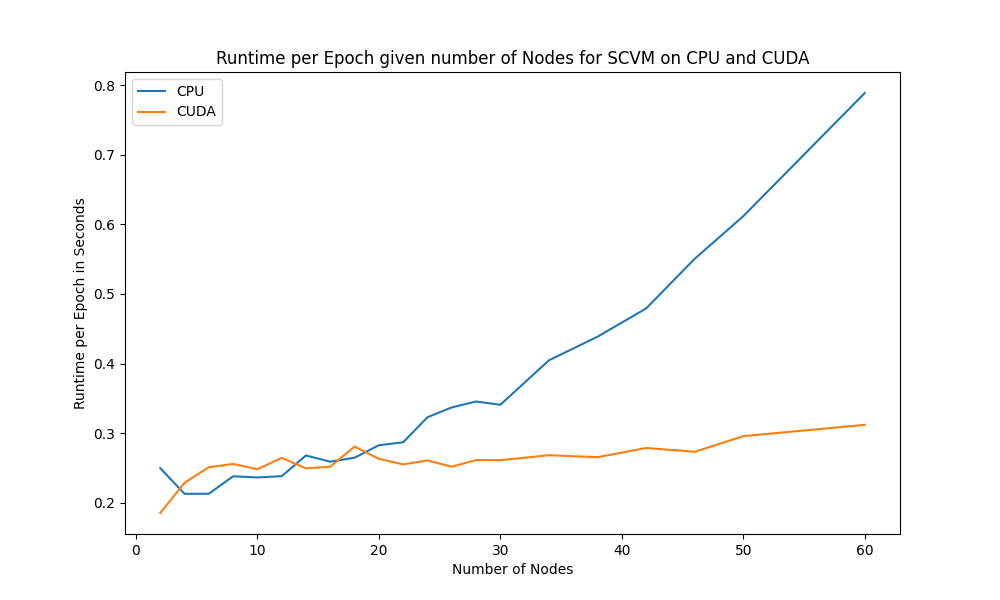
\includegraphics[width=\textwidth]{0_images/numnodes_runtime2.png}
    \caption{Run time of the SCVM relative to the number of nodes $N$}
    \label{fig:NumNodesRuntimes}
\end{figure}
\vspace*{-1cm}
\noindent
The figure depicts a clear difference in run times between using the CPU and CUDA.
They both have similar run times for lower $N$'s, but as the number increases, the run times for the CPU increase at what could look like an exponential growth, while the GPU has a slight linear increase.
It can hence be stated that running on CUDA outperforms CPU for larger dynamic networks.
\\\\
\textbf{Number of Steps}
\\
The second test is carried out in order to evaluate the impact on run time in relation to the number of steps the SCVM has to fit.
For this test, the number of steps is taken from the range:
\begin{equation*}
    \hspace*{-0.8cm} Num_{steps} = [4,8,12,16,20,30,40,50,75,100,150,200,250,300,350,400,450,500,750,1000]\hspace*{-0.5cm}
\end{equation*}
The dataset is generated using $\beta = 5.0$ and $N = 4$ nodes, and the resulting dataset has size $n = 5997$.
Again, for each number of steps, the mean run time per epoch over five runs are recorded for both the CPU and CUDA.
Figure \ref{fig:NumStepsRuntimes} below shows the run times per epoch given the number of steps the SCVM has to fit, using the CPU (in blue) and CUDA (in orange).
\vspace*{-0.2cm}
\begin{figure}[H]
    \centering
    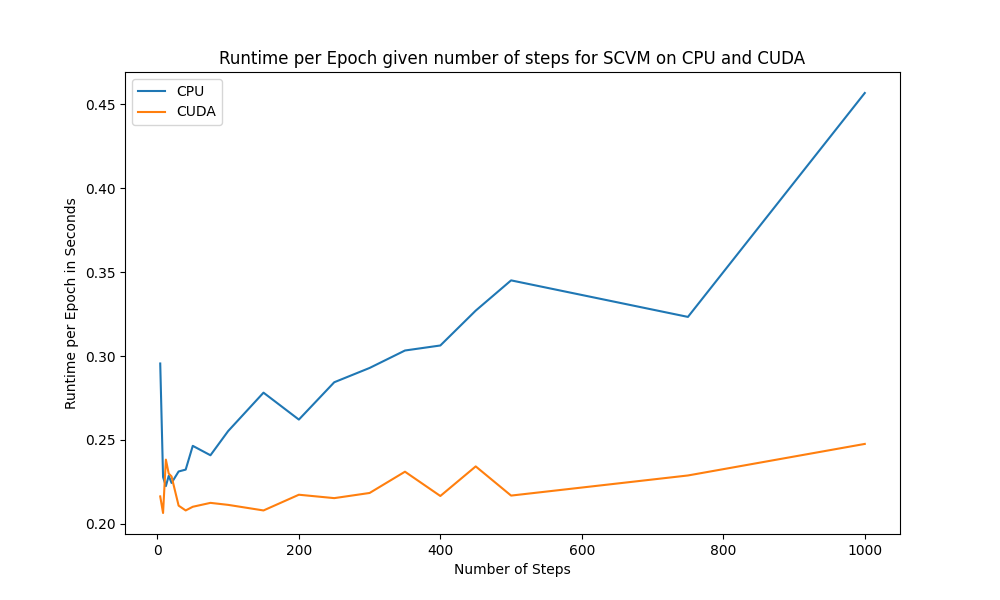
\includegraphics[width=\textwidth]{0_images/steps_runtime2.png}
    \caption{Run time of the SCVM relative to the number of steps}
    \label{fig:NumStepsRuntimes}
\end{figure}
\vspace*{-0.2cm}
\noindent
The increase in run time in relation to the number of steps depicted above, shows the CPU once again being outperformed by CUDA.
The run times increase seemingly linearly for both, but with a lower rate for the CUDA.
\\\\
\textbf{Number of Interactions}
\\
The third and final scalability test is carried out with the goal of evaluating the impact on run time the dataset size has.
For this test, the data is generated based on the $\beta$-value, taken from the range:
\begin{equation*}
    \beta = [5.0, 5.25, 5.5, 5.75, 6.0, 6.25, 6.5, 6.75, 7.0, 7.25, 7.5, 7.75, 8.0, 8.25, 8.5, 8.75, 9.0]
\end{equation*}
The number of interactions generated from these beta values are as follows:
\begin{align*}
    n = [5997, 7997, 10249, 13006, 16387, 21098, 27485, 35269, 45884, 59057, 75356, 
    \\96779, 125039, 160282, 205495, 261802, 338322]
\end{align*}
\noindent
The dataset is generated using $N = 4$ nodes, and SCVM has to fit four velocity vectors to each node, ie. four steps.
Once again, for each dataset size, the mean run time per epoch over five runs are recorded for both the CPU and CUDA.
Figure \ref{fig:NumInteractionsRuntimes} below shows the run times per epoch given the number of steps the SCVM has to fit, using the CPU (in blue) and CUDA (in orange).

\begin{figure}[H]
    \centering
    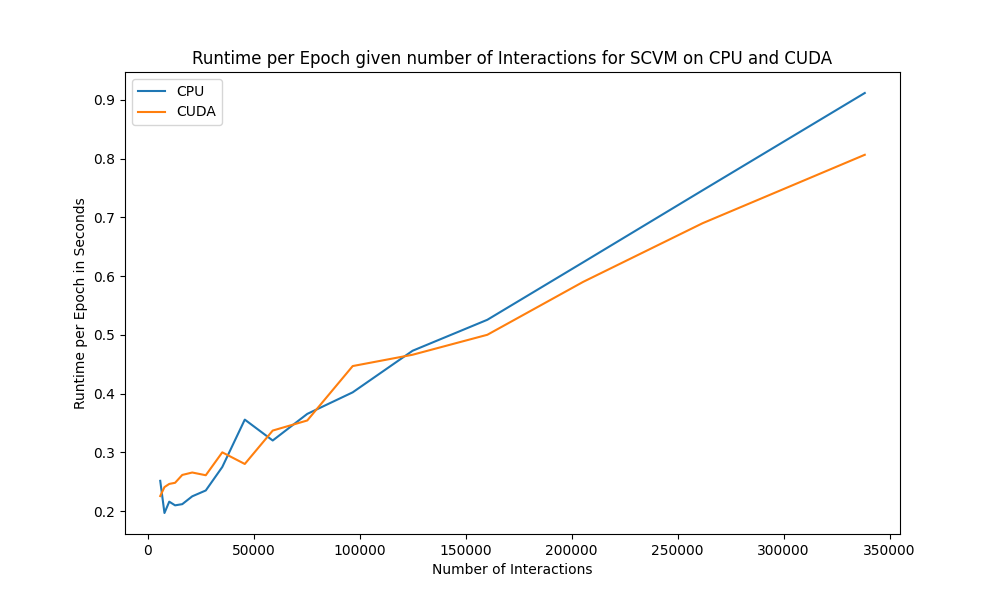
\includegraphics[width=\textwidth]{0_images/numinteractions_runtime2.png}
    \caption{Run time of the SCVM relative to the number of interactions}
    \label{fig:NumInteractionsRuntimes}
\end{figure}
\noindent
The figure above shows similar run times for both the CPU and CUDA in relation to the number of interactions in the dataset.
The growth that they both experience is linear, and hence directly proportional to $n$.